% Created 2021-01-24 Sun 22:50
% Intended LaTeX compiler: pdflatex
\documentclass[11pt]{article}
\usepackage[utf8]{inputenc}
\usepackage[T1]{fontenc}
\usepackage{graphicx}
\usepackage{grffile}
\usepackage{longtable}
\usepackage{wrapfig}
\usepackage{rotating}
\usepackage[normalem]{ulem}
\usepackage{amsmath}
\usepackage{textcomp}
\usepackage{amssymb}
\usepackage{capt-of}
\usepackage{hyperref}
\usepackage{minted}
\hypersetup{colorlinks=true, linkcolor=black, filecolor=red, urlcolor=blue}
\usepackage[turkish]{babel}
\author{Eren Hatırnaz}
\date{8 Aralık 2019}
\title{Yazılım Gündemi - 20\\\medskip
\large 2-8 Aralık 2019}
\hypersetup{
 pdfauthor={Eren Hatırnaz},
 pdftitle={Yazılım Gündemi - 20},
 pdfkeywords={},
 pdfsubject={},
 pdfcreator={Emacs 27.1 (Org mode 9.3)},
 pdflang={Turkish}}
\begin{document}

\maketitle
\tableofcontents \clearpage\shorthandoff{=}

\begin{center}
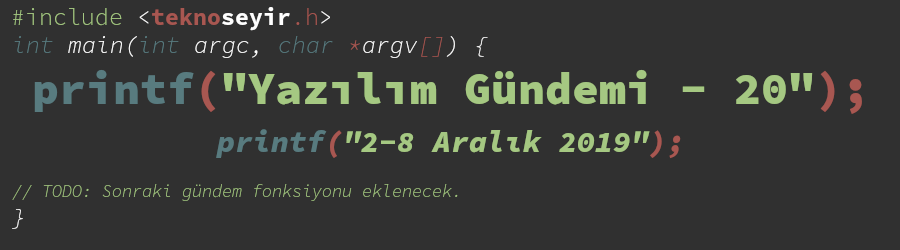
\includegraphics[width=.9\linewidth]{gorseller/yazilim-gundemi-banner.png}
\end{center}

\begin{center}
\href{../19/yazilim-gundemi-19.pdf}{< Önceki Gündem} | \textbf{2-8 Aralık 2019} | \href{../21/yazilim-gundemi-21.pdf}{Sonraki Gündem >}

\href{https://teknoseyir.com/blog/yazilim-gundemi-20-2-8-aralik-2019}{TeknoSeyir'de Oku}
\end{center}

\section{2 zararlı Python kütüphanesi PyPI üzerinden \href{https://www.zdnet.com/article/two-malicious-python-libraries-removed-from-pypi/}{kaldırıldı}}
\label{sec:org1de380c}
Gün geçmiyor ki kişilerin dikkatsizliklerini suistimal eden zararlı yazılımlar
gün yüzüne çıkmasın. Genelde uygulamalar ve hizmetlerde görmeye alıştığımız
fakat son zamanlarda programlama kütüphanelerinde de yayılmakta olan bu tarz
kötü amaçlı kodlar içeren kütüphaneler gittikçe daha ciddi bir tehdit
oluşturmaya başladı. Bu sefer de kütüphane isimlerinde bir benzerlik hilesi
yaparak kendini başka bir kütüphane gibi gösteren ama aslında zararlı kodlar
içeren 2 Python kütüphanesi tespit edildi ve Python paket yöneticilerinin
kullandığı Python Package Index (PyPI) sisteminden kaldırıldı. Kütüphaneler
bunlar:
\begin{itemize}
\item Gerçek kütüphane: \href{https://pypi.org/project/python-dateutil/}{dateutil}. Sahtesi: \href{https://pypi.org/project/python3-dateutil/}{python3-dateutil}.
\item Gerçek kütüphane: \href{https://pypi.org/project/jellyfish/}{jellyfish}. Sahtesi: \href{https://pypi.org/project/jeIlyfish/}{jeIlyfish} (ilk L harfi aslında bir I
harfi).
\end{itemize}
İki sahte kütüphane de aynı kişi tarafından geliştirilmiş ve aslında zararlı
kodları içeren kütüphane jeIlyfish olan, diğerinde ise bu kütüphane içindeki
zararlı dosyayı indirip çalıştıran kodlar mevcut. Zararlı kodların amacı ise
çalıştırıldığı bilgisayardaki SSH ve GPG anahtarlarını çalmak. python3-dateutil
sahte kütüphanesi 29 kasımda yayınlanmış fakat diğeri 1 yıldır (11 Aralık 2018)
yayındaymış.

İki kütüphane de artık erişilemez durumda fakat siz projenize eklemişseniz
elbette otomatik olarak silinmeyecek, bu yüzden Python ile geliştirdiğiniz
projelerinizi bir gözden geçirmenizde fayda var. Her ne kadar dikkatli olmaya
çalışsak da bu tarz güvenlik zafiyetleri maalesef bir anlık dikkatsizliğimizi
bile çok iyi kullanıyor. Bir kere böyle bir kütüphaneyi bağımlılık olarak
eklediysek sonrasında fark etmemiz çok zor oluyor. O yüzden "ben yemem böyle
şeyleri" dememek gerek.
\section{WebAssembly artık W3C onaylı bir \href{https://www.w3.org/2019/12/pressrelease-wasm-rec.html.en}{web standardı oldu}}
\label{sec:org3f7b3a4}
\begin{center}
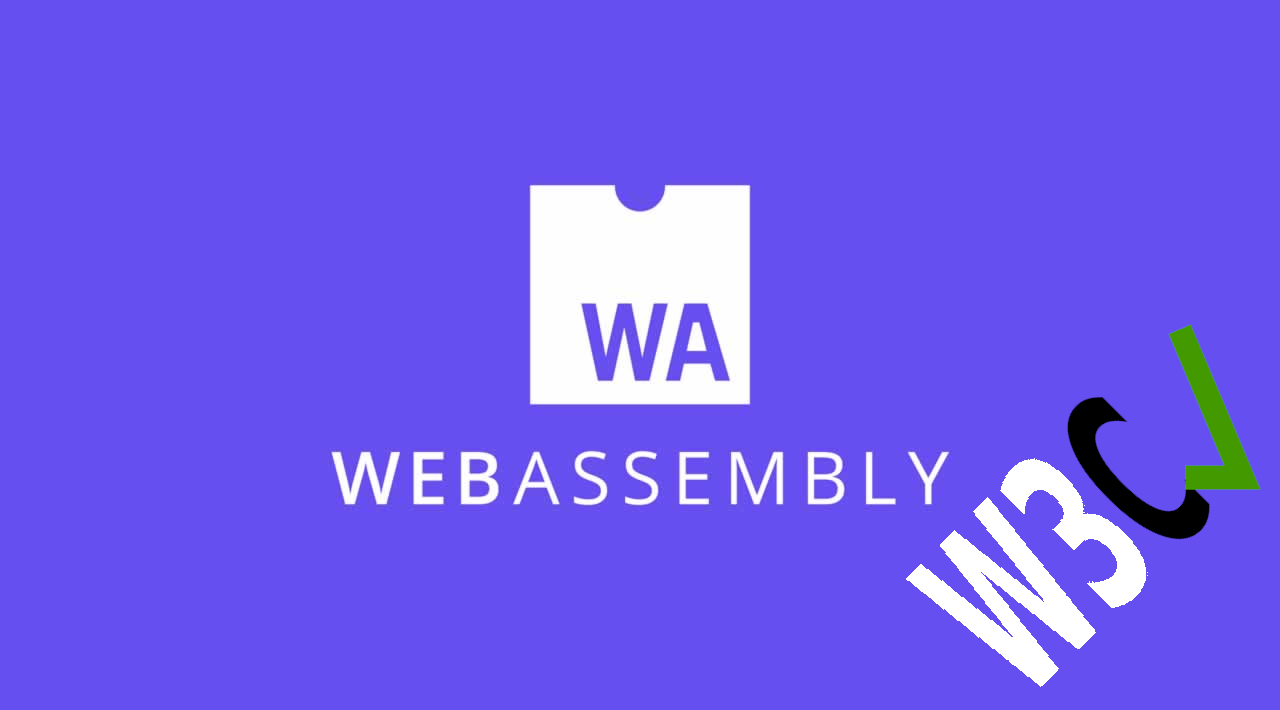
\includegraphics[height=3cm]{gorseller/webassembly-w3c.png}
\end{center}

Her ne kadar alternatifleri çıksa da, zamanla bir şekilde hepsini geride
bırakmış bir dil olan JavaScript uzun zamandır hayatımızda. Fakat son yıllarda
JavaScript'in tahtı yavaş yavaş sallanmaya başlamıştı ve artık kendi
kategorisinde tek dil değil. Çoğumuzun mutlaka ismini en az bir kere duyduğu
WebAssembly, bu hafta içerisinde JavaScript'den sonraki dördüncü Web Standartı
oldu. "Web Standartı" dediğimize göre hepimiz biliyoruz ki bunu ilan
edebilecek bir kurum var: World Wide Web Consortium, çoğumuzun bildiği
şekliyle nam-ı diğer W3C.

Konu başlığına eklediğim bağlantıdaki basın bülteninin yayınlanmasıyla
tarayıcı üzerinde çalışabilen yeni bir W3C onaylı programlama dilimiz oldu
(aslında uzun bir süredir vardı fakat artık resmi olarak onaylı). Tüm yazılım
camiasına hayırlı uğurlu olsun. Elbette WebAssembly sadece tarayıcı üzerinde
çalışan bir dil değil, kendisiyle başka çeşit çeşit işler de yapmak mümkün.
Ayrıca yine W3C geliştiricilere hız ve verimlilik için \href{https://www.w3.org/blog/news/archives/8123}{WebAssembly öneriyor}.

Bu basın bülteninin yayınlanmasının bir diğer anlamı ise artık tarayıcıların
WebAssembly diline destek vermek için büyük bir nedeni var. Benim tahminim
önümüzdeki aylar içerisinde tarayıcılar WebAssembly diline daha büyük
yatırımlar yapacak ve birer birer desteklerini duyuracaklardır. Böylece benim
de WebAssembly hakkında araştırmalar ve denemeler yapmak için bir motivasyonum
oldu. Şimdiye kadar pek detaylıca incelemediğim bu dili daha iyi inceleme
vakti gelmiş.

Siz WebAssembly hakkında ne düşünüyorsunuz? Deneme ve araştırma imkanınız oldu
mu? Olduysa deneyimlerinizi ve görüşlerinizi yorumlar bölümünde
belirtebilirsiniz.
\section{AWS, kodlarımızı inceleyecek \href{https://aws.amazon.com/about-aws/whats-new/2019/12/aws-announces-amazon-codeguru-for-automated-code-reviews-and-application-performance-recommendations/}{yapay zeka hizmetini duyurdu}: \href{https://aws.amazon.com/tr/codeguru/}{Amazon CodeGuru}}
\label{sec:orgfa6e881}
Amazon Web Services (AWS) girenin içerisinden kolay kolay çıkamadığı dev bir
ekosistem. Bu ekosistem bu hafta içerisinde daha da genişledi ve içerisine yeni
onlarca servis eklendi fakat ben bunlardan biriyle ilgili konuşmak istiyorum.
Evet, başlıkta da ismi olan Amazon CodeGuru servisinden bahsediyorum. Bu servis
sizin kodlarınızı inceleyerek size çeşitli önerilerde bulunan eğitilmiş bir
yapay zeka. Şu an Preview olarak bazı bölgelerde kullanımda açılmış.

Günümüzde gerek teknolojik gelişmelerin hızlanması gerekse de bilgisayar
sistemlerinin verimliliğinin artmasıyla bazı mesleklerin yerini yapay zeka
sistemlerinin alacağı öngörüleri fazlaca yaygın. Bu yapay zeka sistemlerini
geliştiren bizler her ne kadar "ya sistemleri biz geliştiriyoruz zaten, bize
bi' şey olmaz", diye düşünsek de, ben aynı fikirde değilim. Günün birinde
birisi mutlaka "kod yazan yapay zeka" sistemi çıkaracaktır ve bu sistem verimli
ve ekonomik olduğu takdirde de bizim pabuçumuzun dama atılması çok kolay. Böyle
bir şeye de çok uzak olduğumuz söylenemez. Bugün de Amazon'un bu hizmeti ile
birlikte bunun mümkünlüğüne daha çok inanmaya başladım.

Yani anlayacağınız \href{https://tr.pinterest.com/pin/363665738639735548/}{çember bizim için de daralıyor} arkadaşlar. Bugün kodlarımızı
inceleyip bize öneri sunan yapay zeka, yarın kod da yazar. Biraz komplo teorisi
vari olacak ama belki de Amazon bu servisi "kod yazan yapay zeka"yı yaratmak
için kullanacak, kim bilir\ldots{} Elbette yine yazılım mesleğinin yerini tamamen
yapay zeka almayacak. Sonuçta bu yapay zekaları geliştirecek olanlar da
bizleriz (gerçi bundan da emin değilim çünkü geçen senelerde bir haftalık
gündem değerlendirmesinde "yapay zekanın geliştirdiği yapay zeka, insanların
geliştirdiği yapay zekadan daha verimli" gibi bir haber dinlediğimi
hatırlıyorum) ama eskiye göre yazılım geliştirici ihtiyacı bir hayli
azalacaktır diye düşünüyorum.

O gün geldiğinde yazılım camiasının vereceği tepkiyi çok merak ediyorum. Şu an
yapay zeka geliştirmeleriyle birçok mesleğin yerini almayı planlayarak sevinen,
"ya benim geliştirdiğim sistem insandan daha verimli çalışıyor işte
istatistikler" diyerek olaya son derece bilimsel yaklaşabilen arkadaşlar, o gün
geldiğinde de acaba "e tabii ki de benden verimliyse buyursun geçsin yerime ben
kenara çekilirim" diyebilecekler mi, yoksa Osmanlı döneminde matbaanın
gelmesini istemeyen hattatlar gibi bir akım mı oluşacak? Benim tahminim
ikincisinin gerçekleşeceği yönünde, çünkü hiç kimse -haklı olarak- mesleğini
kolay kolay bırakmak istemez. Fakat artık Osmanlı döneminde değiliz, böyle bir
sistem ekonomik ve verimli olduğu takdirde hiçbir işveren bizim göz yaşımıza
bakmaz. Fazla mesai ücreti vermeden (gerçi Türkiye'de zaten alamıyoruz ama)
7/24 çalıştırabileceği bir yapay zeka varken niye bize maaş ödesin?!

Bu konuda siz ne düşünüyorsunuz arkadaşlar? Özellikle bu konu hakkında
görüşlerini çok merak ediyorum. Lütfen okuyorsanız fikirlerinizi belirtmekten
kendinizi geri koymayın. Yorumlar bölümünde konuşalım.

Ayrıca Amazon'un tanıttığı diğer hizmetlerin birkaçı da bu şekilde (gözden
kaçırdıklarım olabilir, takip etmek çok zor):
\begin{itemize}
\item \href{https://aws.amazon.com/tr/blogs/aws/amazon-braket-get-started-with-quantum-computing/}{Amazon Braket – Quantum Computing}
\item \href{https://aws.amazon.com/tr/blogs/aws/new-amazon-managed-apache-cassandra-service-mcs/}{Amazon Managed Apache Cassandra Service (MCS)}
\item \href{https://aws.amazon.com/tr/blogs/aws/amazon-sagemaker-autopilot-fully-managed-automatic-machine-learning/}{Amazon SageMaker Autopilot – Automatically Create High-Quality}
\item \href{https://aws.amazon.com/tr/kendra/}{Amazon Kendra – Enterprise Search Service}
\item \href{https://aws.amazon.com/tr/blogs/aws/identify-unintended-resource-access-with-aws-identity-and-access-management-iam-access-analyzer/}{AWS Identity and Access Management (IAM) Access Analyzer}
\item \href{https://aws.amazon.com/tr/ec2/nitro/nitro-enclaves/}{AWS Nitro Enclaves - Isolated Compute Environments}
\item \href{https://aws.amazon.com/tr/fraud-detector}{Amazon Fraud Detector}
\end{itemize}
\section{JetBrains takımlar için yeni bir \href{https://blog.jetbrains.com/blog/2019/12/05/welcome-to-space/}{ürün tanıttı}: \href{https://www.jetbrains.com/space/}{Space}}
\label{sec:org30ef832}
JetBrains firmasını çoğumuz, hemen her programlama dili için çıkardıkları IDE
araçları ve Kotlin programlama dili ile tanıyoruz. Bu sefer programlama
dillerinden ziyade daha çok şirketlerdeki geliştirici takımları çıkardıkları
bir ürünün erken erişim programını duyurumalarıyla gündemimizde yer alıyorlar.
Git bazlı versiyon kontrol, bloglar, planlama, code review süreçleri vb. gibi
birçok özellik ile birlikte gelen bu ürünü hem servis olarak JetBrains
üzerinden kullanabiliyorsunuz, hem de kurumsal firmalar için kendi sunucunuzda
barındırabiliyorsunuz.

Daha detaylı bilgi için konu başlığına eklediğim bağlantılara tıklayabilir ya
da \href{https://www.youtube.com/watch?v=t1vMUV9jYRs}{şuradaki duyuru videosunu izleyebilirsiniz}.
\section{Django 3.0 sürümü \href{https://docs.djangoproject.com/en/3.0/releases/3.0/}{yayınlandı}}
\label{sec:org79b563a}
Popüler Python web framework'ü Django'nun 3.0 sürümü yayınlandı. Bu yeni Django
sürümü Python 3.6, 3.7 ve 3.8 sürümlerini destekliyor. Django geliştiricileri,
üçüncü parti kütüphane geliştiricilerine Django 2.2'den önceki tüm sürümlere
destek vermeyi durdurmayı tavsiye etmişler. Bu sürümde gelen yeniliklerin
birkaçı ise şu şekilde:
\begin{itemize}
\item MariaDB desteği,
\item \href{https://asgi.readthedocs.io/en/latest/}{ASGI (Asynchronous Server Gateway Interface)} desteği,
\item Diğer özellikler için konu başlığına eklediğim bağlantıya tıklayabilir ya
da \href{https://www.youtube.com/watch?v=\_BBNVFirvTY}{şuradaki videoyu izleyebilirsiniz}.
\end{itemize}

Ayrıca Django sürüm yükseltme rehberi için \href{https://docs.djangoproject.com/en/3.0/howto/upgrade-version/}{buraya} tıklayabilirsiniz.
\section{PHP Versiyonları İstatistikleri \href{https://blog.packagist.com/php-versions-stats-2019-2-edition/}{2019.2 yayınlandı}}
\label{sec:org04042b4}
\begin{figure}[htbp]
\centering
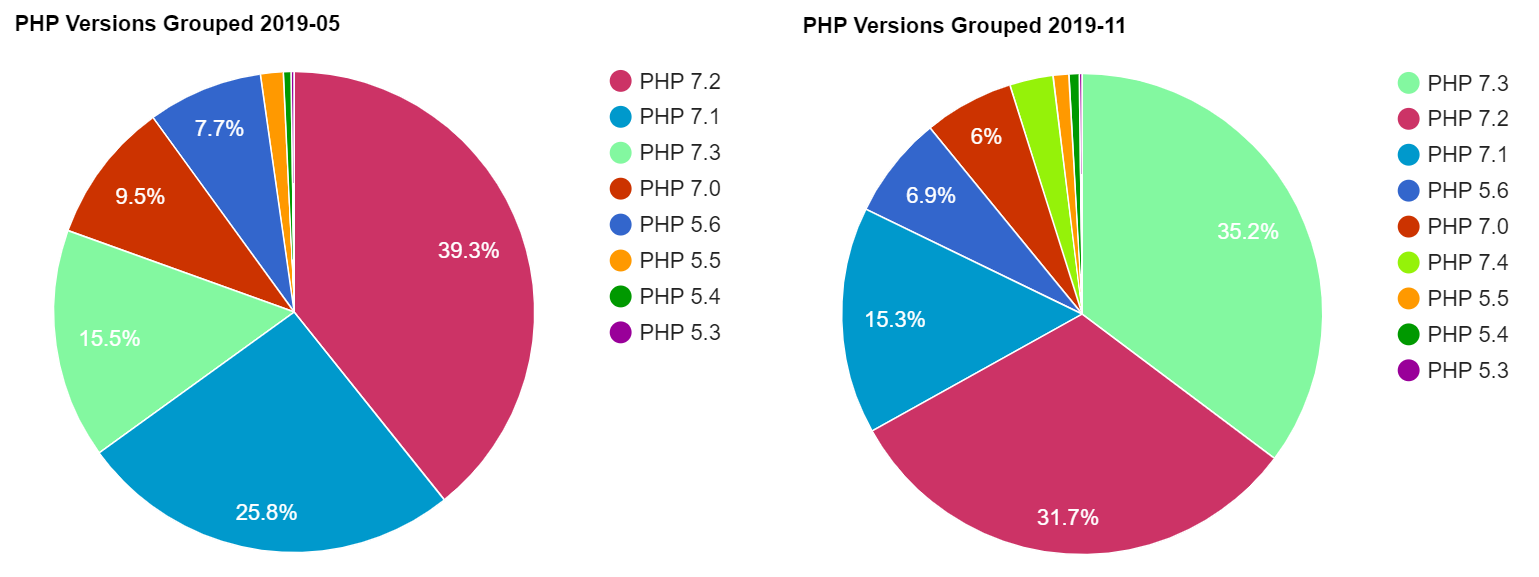
\includegraphics[width=.9\linewidth]{gorseller/php-versiyon-1.png}
\caption[\textbf{(SOL):}]{\textbf{(SAĞ):} Mayıs 2019 PHP Versiyonları Kullanım Oranları \\
 \textbf{(SOL):} Kasım 2019 PHP Versiyonları Kullanım Oranları}
\end{figure}

\begin{figure}[htbp]
\centering
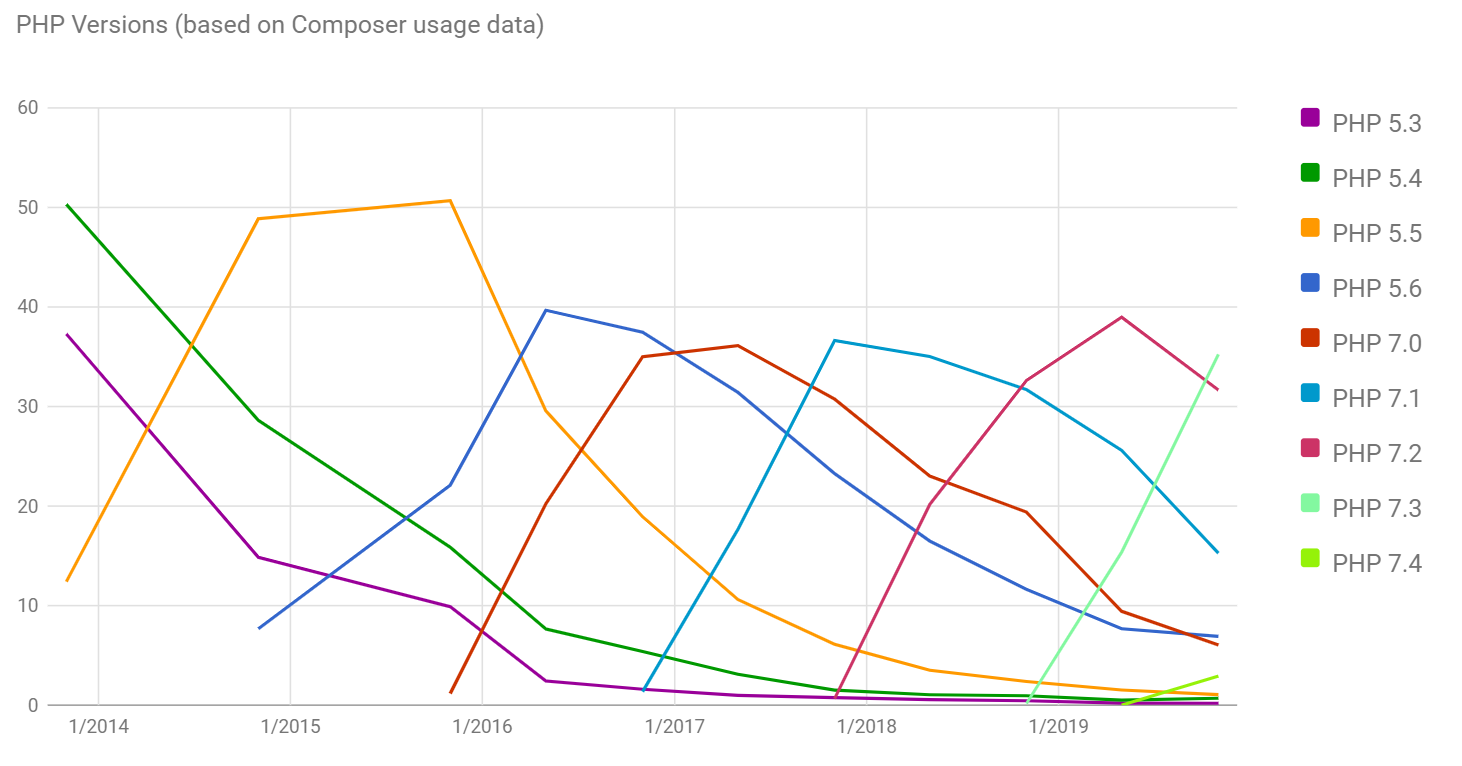
\includegraphics[width=.9\linewidth]{gorseller/php-versiyon-2.png}
\caption{Composer kullanım verilerine göre PHP versiyonlarının zamanda değişen kullanım	oranları}
\end{figure}

\newpage
\section{Qt yeni eklenti mağazasını \href{https://www.qt.io/blog/qt-marketplace}{duyurdu}: \href{https://marketplace.qt.io/}{Qt Marketplace}}
\label{sec:org30b1f9c}
C++ ile platformlar-arası (cross-platform) uygulama geliştirmeye yarayan Qt
uygulama çatısının artık bir eklenti mağazası var. Geliştiriciler ücretli ya da
ücretsiz birçok eklentisi bu mağaza üzerinden alıp, doğrudan uygulamaları
üzerinde kullanabilecekler.
\section{Yaklaşan Etkinlikler}
\label{sec:org6b35be6}
\begin{longtable}{|p{8cm}|l|l|}
\hline
Etkinlik İsmi & Yeri & Tarihi\\
\hline
\endfirsthead
\multicolumn{3}{l}{Önceki sayfadan devam ediyor} \\
\hline

Etkinlik İsmi & Yeri & Tarihi \\

\hline
\endhead
\hline\multicolumn{3}{r}{Devamı sonraki sayfada} \\
\endfoot
\endlastfoot
\hline
\href{https://www.eventbrite.com/e/tersine-muhendislik-workshop-tickets-84404653591}{Tersine Mühendislik - Workshop} & İstanbul & 10 Aralık 18:30\\
\href{https://www.meetup.com/tr-TR/Istanbul-Java-User-Group/events/265809996/}{Future of Java Virtual Machines and Frameworks - GraalVM and Quarkus} & İstanbul & 10 Aralık 19:00\\
\href{https://www.meetup.com/tr-TR/TestHive/events/266285658/}{Test Automation with Taiko} & İstanbul & 10 Aralık 19:30\\
\href{https://www.meetup.com/tr-TR/ING-\%25C4\%25B0novasyon-Merkezi/events/266930475/}{LearnDocker İstanbul: Docker'a Giriş} & İstanbul & 11 Aralık 18:30\\
\href{https://www.meetup.com/tr-TR/Oracle-Developer-Meetup-Istanbul/events/266783829/}{Oracle Developer Meetup} & İstanbul & 11 Aralık 18:45\\
\href{https://www.meetup.com/tr-TR/Docker-Istanbul/events/266413178/}{LearnDocker İstanbul: Docker'a Giriş - Uygulamalı} & İstanbul & 11 Aralık 19:00\\
\href{https://www.meetup.com/tr-TR/DL\_Experts\_Ist/events/266781111/}{DL Exerts - \#1 : Introduction to TensorFlow 2.0} & İstanbul & 11 Aralık 19:00\\
\href{https://www.eventbrite.com/e/siber-olaylarda-5n1k-yeterli-mi-hacknightsorg-tickets-78022424171}{Siber Olaylarda 5N1K Yeterli Mi?} & Ankara & 12 Aralık 19:00\\
\href{https://www.meetup.com/tr-TR/Emlakjet-Engineering/events/266403417/}{Introduction to Tensorflow 2.0} & İstanbul & 12 Aralık 19:00\\
\href{https://www.eventbrite.com/e/kuantum-programlama-uygulamalar-hackathonu-tickets-84534931255}{Kuantum Programlama Uygulamaları Hackathonu} & Ankara & 14 Aralık 09:00\\
\href{https://www.meetup.com/tr-TR/JAMstack/events/266280664/}{JAMstack Istanbul Coffee Talk - 4} & İstanbul & 14 Aralık 13:00\\
\href{https://www.eventbrite.com/e/yapay-zeka-ve-hukuk-zirvesi-tickets-84402900347}{Yapay Zeka ve Hukuk Zirvesi} & İstanbul & 16 Aralık 09:00\\
\href{https://www.meetup.com/tr-TR/AWS-User-Group-Turkey/events/266942291/}{AWS Meetup 44 - Re: Invent Yeni Servisler ve Gelişmeler} & İstanbul & 16 Aralık 19:00\\
\href{https://www.meetup.com/tr-TR/Software-Craftsmanship-Turkey/events/262170141/}{Software Craftsmanship Turkey Meetup} & İstanbul & 18 Aralık 19:00\\
\href{https://www.meetup.com/tr-TR/GDG-Manisa/events/266749804/}{GDG DevFest Manisa 19'} & Manisa & 19 Aralık 09:30\\
\href{https://www.eventbrite.com/e/hakan-erdogan-ile-developer-muhabbeti-facebook-devc-istanbul-tickets-85326589125}{Hakan Erdoğan ile Developer Muhabbeti} & İstanbul & 19 Aralık 18:30\\
\href{https://www.eventbrite.com/e/windows-forensics-hacknightsorg-tickets-78022654861}{Windows Forensics} & Ankara & 19 Aralık 19:00\\
\href{https://kommunity.com/devnot-yazilimci-bulusmalari/events/yazilim-sektorunde-serbest-danisman-olarak-calismak}{Yazılım Sektöründe Serbest Danışman Olarak Çalışmak} & İstanbul & 20 Aralık 19:00\\
\href{https://kommunity.com/frontend-istanbul/events/tatilcomun-monolotik-uygulamadan-spaya-gecis-oykusu}{Tatil.com’un Monolitik Uygulamadan SPA’ya Geçiş Öyküsü} & İstanbul & 20 Aralık 19:30\\
\href{https://www.meetup.com/tr-TR/istanbul-yapay-zeka-toplulugu/events/267007562/}{TensorFlow 2.0 Atölyesi} & İstanbul & 22 Aralık 15:00\\
\hline
\end{longtable}
\section{Diğer Haberler}
\label{sec:org7466864}
\begin{itemize}
\item Microsoft, Rust benzeri yeni bir güvenlik odaklı dil \href{https://www.zdnet.com/article/microsoft-were-creating-a-new-rust-based-programming-language-for-secure-coding/}{üzerinde çalışıyormuş}
\item .Net Core 3.1 \href{https://devblogs.microsoft.com/dotnet/announcing-net-core-3-1/}{duyuruldu}.
\item Netflix, gerçek zamanlı veri bilimi aracını \href{https://medium.com/netflix-techblog/open-sourcing-metaflow-a-human-centric-framework-for-data-science-fa72e04a5d9}{açık kaynak yaptı}: \href{https://metaflow.org/}{Metaflow},
\href{https://github.com/Netflix/metaflow}{GitHub Deposu}.
\item Rust, 2019 yılı durumu için anket \href{https://blog.rust-lang.org/2019/12/03/survey-launch.html}{başlattı}: \href{https://docs.google.com/forms/d/e/1FAIpQLSdu9oHszoG4CAq1X1FkJIp70bXSbMNKIP0n4Serr\_gTszl01Q/viewform}{2019 State of Rust Language
Survey}, \href{https://github.com/rust-community/team/wiki/State-of-the-Rust-Language-Community-Survey-FAQ}{SSS}
\item Mozilla'nın sesten yazı elde etme motoru \href{https://hacks.mozilla.org/2019/12/deepspeech-0-6-mozillas-speech-to-text-engine/}{DeepSpeech 0.6 sürümüne ulaştı}.
\href{https://github.com/mozilla/DeepSpeech/releases/tag/v0.6.0}{Değişiklik Notları}.
\item Onaylanan bir Pull Request GitHub'ın geçici olarak \href{https://github.com/ianstormtaylor/slate/pull/3093\#issuecomment-559313932}{çökmesine neden oldu}.
\item React projeleri oluşturmaya yarayan \href{https://github.com/facebook/create-react-app}{create-react-app} aracının 3.3.0 sürümü
\href{https://github.com/facebook/create-react-app/releases/tag/v3.3.0}{yayınlandı}.
\item Go programlama dilinin \href{https://golang.org/doc/devel/release.html\#go1.13.minor}{3.13.5} ve \href{https://golang.org/doc/devel/release.html\#go1.12.minor}{3.12.14} sürümleri yayınlandı.
\item Android geliştirme araçlarında güncellemeler:
\begin{itemize}
\item \href{https://androidstudio.googleblog.com/2019/12/android-studio-40-canary-5-available.html}{Android Studio 4.0 Canary 5}
\item \href{https://androidstudio.googleblog.com/2019/12/android-studio-36-beta-5-available.html}{Android Studio 3.6 Beta 5}
\item \href{https://androidstudio.googleblog.com/2019/12/android-studio-353-available.html}{Android Studio 3.5.3}
\item \href{https://androidstudio.googleblog.com/2019/12/emulator-29212-to-canary.html}{Emulator 29.2.12 Canary}
\end{itemize}
\item Birçok AndroidX API'sine \href{https://developer.android.com/jetpack/androidx/versions/all-channel\#december\_4\_2019}{güncelleme geldi}. \href{https://mobile.twitter.com/ianhlake/status/1202322055124750337}{Twitter}
\item Google, Kotlin ile yola \href{https://android-developers.googleblog.com/2019/12/androids-commitment-to-kotlin.html}{devam ediyor}.
\item JetBrains Academy platformuna Kotlin \href{https://blog.jetbrains.com/blog/2019/12/05/jetbrains-academy-kotlin/}{içerikleri eklendi}
\item KotlinConf 2019'da Kotlin 1.4 ile gelecek bazı yeniliklerden \href{https://blog.jetbrains.com/kotlin/2019/12/what-to-expect-in-kotlin-1-4-and-beyond/}{bahsedildi}.
\item Certbot Beta'dan çıktı ve 1.0 ile stabil \href{https://www.eff.org/deeplinks/2019/12/certbot-leaves-beta-release-10}{sürüme ulaştı}.
\item GitClear, proje keşfetmeyi kolaylaştırmak için bir \href{https://www.gitclear.com/blog/introducing\_open\_repos\_a\_free\_product\_to\_aid\_open\_source\_development}{beta özellik duyurdu}:
\href{https://www.gitclear.com/open\_repos}{Open Repos}.
\item Rust ve WebAssemby ile geliştirilmiş yeni bir ön-yüz kütüphanesi \href{https://blog.anp.lol/rust/moxie-intro/}{duyuruldu}:
\href{https://github.com/anp/moxie}{moxie}.
\item Uygulamalar için sanal sunucu olan GraalVM, WebAssembly desteğini \href{https://medium.com/graalvm/announcing-graalwasm-a-webassembly-engine-in-graalvm-25cd0400a7f2}{duyurdu}:
\href{https://github.com/oracle/graal/tree/master/wasm}{GraalWasm}.
\item Jupyter Notebooks ile kütüphane geliştirmeye yarayan yeni bir araç
\href{https://www.fast.ai/2019/12/02/nbdev/}{duyuruldu}: \href{https://nbdev.fast.ai/}{nbdev}, \href{https://github.com/fastai/nbdev}{GitHub Deposu}.
\item PHP Statik analiz aracı PHPStan'ın 0.12 sürümü \href{https://medium.com/ondrejmirtes/phpstan-0-12-released-f1a88036535d}{yayınlandı}.
\item Çevrimiçi editör Gitpod'a, GitLab \href{https://www.gitpod.io/blog/gitlab-support/}{desteği eklendi}.
\item Notepad++ 7.8.2 "Free Uyghur Edition" sürümü \href{https://notepad-plus-plus.org/news/v782-free-uyghur-edition/}{yayınlandı}.
\item C++ ağ kütüphanesi \href{https://github.com/seladb/PcapPlusPlus}{PcapPlusPlus}, v19.12 sürümünü \href{https://github.com/seladb/PcapPlusPlus/releases/tag/v19.12}{duyurdu}.
\item Bettendar 1.0 sürümü \href{https://bottender.js.org/blog/2019/12/05/bottender-1}{duyuruldu}.
\item OpenAPIGenerator 4.2.2 sürümü \href{https://github.com/OpenAPITools/openapi-generator/releases/tag/v4.2.2}{yayınlandı}.
\item Tera 1.0 \href{https://www.vincentprouillet.com/blog/tera-v1-is-here/}{yayınlandı}.
\item uvw 2.3.0 sürümü \href{https://github.com/skypjack/uvw/releases/tag/v2.3.0\_libuv-v1.34}{çıktı}.
\item WT \& JWT 3.5.0 ve WT 4.2.0 sürümleri \href{https://www.webtoolkit.eu/wt/news/2019/12/03/wt\_\_\_jwt\_3\_5\_0\_and\_wt\_4\_2\_0}{çıktı}.
\item Keigen 1.6.0 sürümü \href{https://github.com/paramsen/Keigen/releases/tag/1.6.0}{çıktı}.
\item Mimalloc Rust 0.1.11 sürümü \href{https://github.com/purpleprotocol/mimalloc\_rust/releases/tag/v0.1.11}{çıktı}.
\item Cap'n Proto for Rust 0.11.0 sürümü \href{https://dwrensha.github.io/capnproto-rust/2019/12/06/async-await.html}{çıktı}.
\item Emacs paketi lsp-mode 6.2 sürümünü \href{https://github.com/emacs-lsp/lsp-mode/blob/master/doc/changelog.org\#release-62}{çıkardı}.
\item Tokio v0.2.3 sürümü \href{https://github.com/tokio-rs/tokio/releases/tag/tokio-0.2.3}{çıktı}.
\end{itemize}
\section{Lisans}
\label{sec:orgea53ec3}
\begin{center}
\begin{center}

\includegraphics[height=1.5cm]{../../../img/CC_BY-NC-SA_4.0.png}
\end{center}

\href{yazilim-gundemi-20.pdf}{Yazılım Gündemi - 20} yazısı \href{https://erenhatirnaz.github.io}{Eren Hatırnaz} tarafından \href{http://creativecommons.org/licenses/by-nc-sa/4.0/}{Creative Commons
Atıf-GayriTicari-AynıLisanslaPaylaş 4.0 Uluslararası Lisansı} (CC BY-NC-SA 4.0)
ile lisanslanmıştır.
\end{center}
\end{document}
